\section{Magnetic Fields}

% Magnetic fields

We are interested in modeling the behaviour of the net magnetization,
$\textbf{M}$, of spin packets under the influence of one or more
magnetic fields. This is a function dependent on the time, $t$, and
position, $\textbf{p}$, within the sample. The functions describing
each coordinate component of $\textbf{M}$ are $M_x$, $M_y$ and
$M_z$. Thus our net magnetization is given by

\begin{displaymath}
  \textbf{M}(t, \textbf{p}) = \langle M_x(t, \textbf{p}), M_y(t, \textbf{p}), M_z(t, \textbf{p}) \rangle
\end{displaymath}

As stated previously, when only the static magnetic field
$\mathbf{B}_0 = \langle 0, 0, B_0 \rangle$ is active, $\textbf{M}$
will lie at equilibrium along the z-axis. Thus $\textbf{M} = \langle
0, 0, M_{eq} \rangle$, where $M_{eq}$ is the magnitude of $\textbf{M}$.

The gyromagnetic ratio, $\gamma$, of a particle is the ratio of it's
magnetic dipole moment to it's angular momentum. This means that
$\gamma$ can tell us how fast the net magnetization will precess
around the magnetic field applied to it. 

\begin{displaymath}
  \omega = \gamma \| \mathbf{B} \|
\end{displaymath}

The gyromagnetic ratio for hydrogen atoms is $42.58 \cdot 10^6 Hz / T$
(hertz pr. tesla).

With this we can now formulate the bloch equations that descripe the
net magnetizations rate of change over time with respect to the sum of
magnetic fields, $\mathbf{B}$.

% Bloch equations
\begin{displaymath}
  \frac{d\mathbf{M}}{dt} = \gamma \mathbf{M} \times \mathbf{B} -
  \frac{\langle M_x, M_y, 0 \rangle}{T_2} - \frac{\langle 0, 0, M_z -
    M_{eq} \rangle}{T_1}
\end{displaymath}

$T_1$ and $T_2$ are relaxation times for the spins. $T_1$ is the
\textit{spin-lattice} relaxation time and describe how fast the net
magnetization will return to equilibrium. $T_2$ is the
\textit{spin-spin} relaxation time and reflects how fast the magnitude
of the net magnetizations transverse components goes to 0. $T_2$ will
always be smaller or equal to $T_1$.

% @TODO figures of relaxation times

% Magnetic fields

As explained earlier $\mathbf{B}$ is the sum of three magnetic fields;
the static field $\mathbf{B}_0$, the RF field $\mathbf{B}_1$ and the
gradient field $\mathbf{B}_G$.

\begin{displaymath}
  \mathbf{B} = \mathbf{B}_0 + \mathbf{B}_1 + \mathbf{B}_G
\end{displaymath}

The static field, as written earlier, is simply $\mathbf{B}_0 =
\langle 0, 0, B_0 \rangle$, which is a magnetic field lying along the
z-axis. $\mathbf{B}_0$ causes the spin of the nuclei to precess about
the z-axis at frequency $\gamma B_0 = \omega_0$.

The RF magnetic field, or RF pulse, $\mathbf{B}_1$ is more complex. It
has to rotate the net magnetization 90 degrees into the transverse
plane, while the aggregate magnetic moment is precessing about the
$\mathbf{B}_0$ field. In order to do that $\mathbf{B}_1$ is itself
rotating about $\mathbf{B}_0$ at frequence $\omega_0$.

\begin{displaymath}
  \mathbf{B}_1 = \langle B_1 cos(\omega_0 t), B_1 sin(\omega_0 t), 0\rangle
\end{displaymath}

The $\mathbf{B}_1$ field does not simply rotate the net magnetization
instantly. Instead it needs to be active at a specific time interval
$\tau_{90\degree}$. The time interval can be calculated using

\begin{displaymath}
  \tau_{90\degree} = \frac{1 / 4}{\gamma * \|\mathbf{B}_1\|}
\end{displaymath}

\subsection{Magnetic field gradients}

\begin{figure}
  \centering
  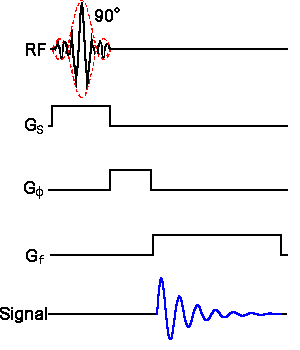
\includegraphics[width=5cm]{gradientSequence}
  \caption{A timing diagram of the application of gradients with
    respect to the RF pulse and signal acquisition.}
  \label{fig:gradientSequence}
\end{figure}

Recall from earlier that if all net magnetizations are spinning in the
same phase and at the same frequency, they are indistinguishable to
the fourier transform and thus produces on image with only one
voxel. We will now in more detail present the gradient fields that
help distinguish the individual spin packets.

We have previously included the gradient fields in our equations as
one variable, $\mathbf{B}_G$. This is purely done to simplify the
equations. In practice one must remember that the gradient field
actually consists of the 3 seperat gradient fields described in
\refsec{sec:MRI}.

\begin{displaymath}
  \mathbf{B}_G = \mathbf{B}_{G_s} + \mathbf{B}_{G_\phi} + \mathbf{B}_{G_f}
\end{displaymath}

As can be seen on \reffig{fig:gradientSequence} the individual
gradients are never active at the same time.

The strenght of all the gradient fields applied are linearly
increasing along a given normal, $\mathbf{G}$, and all gradient fields
have the same direction as $\mathbf{B}_0$. The generel equation for a
gradient field thus becomes.

\begin{displaymath}
  \mathbf{B}_G(\mathbf{p}) = \langle 0, 0, \mathbf{G} \cdot \mathbf{p} \rangle
\end{displaymath}


The first gradient field that is applied is the slice selection
gradient, which is active together with the RF field. As previously
described $\mathbf{B}_{G_s}$ is responsable for ensuring that only a
slice through the patient is affected by the RF pulse and thus that
only this slice will produce a signal. In the theory behind MRI this
slice is placed in the xy-plane with a normal $\langle 0, 0, G_s
\rangle$ and the gradient field is therefore

\begin{displaymath}
  \mathbf{B}_{G_s}(\mathbf{p}) = \langle 0, 0, G_s p_z \rangle
\end{displaymath}


% The y-axis is the phase encode direction and is phase encoded with a
% phase gradient.

The next gradient field applied is phase encoding gradient,
$\mathbf{B}_{G_\phi}$. This is applied to distinguish rotations along
the y-axis and therefore has the form

\begin{displaymath}
  \mathbf{B}_{G_\phi}(\mathbf{p}) = \langle 0, 0, G_\phi p_y \rangle
\end{displaymath}

\begin{figure}
  \centering
  \subfigure[In phase.]{
    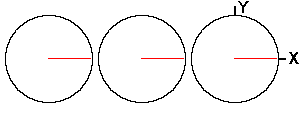
\includegraphics[width=5cm]{inPhase}
  }
  \subfigure[Out of phase.]{
    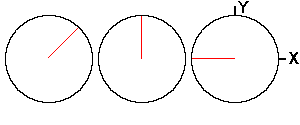
\includegraphics[width=5cm]{outOfPhase}
  }
  \caption{Figures of in-phase and phase shifted net
    magnetizations. Here the phase shift is along the x-axis.}
  \label{fig:phaseShift}
\end{figure}

With the phase encoding gradient active, each net magnetization vector
along the y-axis will precess at it's own unique larmor frequency. 

\begin{displaymath}
  \omega_\phi(\mathbf{p}) = \gamma (B_0 + B_{G_\phi} \cdot p_y)
\end{displaymath}

It therefore follows that when the phase encode gradient is turned
off, all the net magnetization vectors will return to precessing at
the same larmor frequency, $\omega_0$, but out of phase with each
other, as can be seen on \reffig{fig:phaseShift}. In
\refsec{sec:imaging} we shall see how this enables the fourier
transform to distinguish spin packets along the y-axis.

To enable the fourier transform to reconstuct the intensity of a given
spin packet, we need the phase encoding oscilate. This is achieved by
letting the strength of the phase gradient, $B_{G_\phi}$, start at
$G_{\phi_{max}}$ for the first slice excitation and then linearly drop to
$-G_{\phi_{max}}$ in the last excitation.

%TODO phase time and calculating strength



% Constant gradient field along the x axis. The strength of the
% gradient field increases along the x-axis and never changes over the
% course of the signal acquisition.

The final gradient field is the frequency encoding gradient that
encodes the signal along the x-axis.

\begin{displaymath}
  \mathbf{B}_{G_f}(\mathbf{p}) = \langle 0, 0, G_f p_x \rangle
\end{displaymath}

The frequency encoding gradient is turned on while aquirering the
data, to give all net magnetizations along the x-axis their own larmor
frequency.

\begin{displaymath}
  \omega_f(\mathbf{p}) = \gamma (B_0 + B_{G_f} \cdot p_x)
\end{displaymath}

TODO time and strength?

While we here have placed all gradient fields along a specific axis in
our coordinate system, one should remember that we are free to place
the coordinate system in any way we like and thus the theory
generalizes to gradients in any direction, which is useful for oblique
image acquisition.






%%% Local Variables:
%%% mode: latex
%%% TeX-master: t
%%% TeX-PDF-mode: t
%%% End:
